%Jennifer Pan, August 2011

\documentclass[10pt,letter]{article}
	% basic article document class
	% use percent signs to make comments to yourself -- they will not show up.

\usepackage{amsmath}
\usepackage{amssymb}
	% packages that allow mathematical formatting

\usepackage{graphicx}
\usepackage{tikz}
	% package that allows you to include graphics

\usepackage{setspace}
	% package that allows you to change spacing

\onehalfspacing
	% text become 1.5 spaced

\usepackage{fullpage}
	% package that specifies normal margins


\begin{document}
	% line of code telling latex that your document is beginning


\title{ECON501 Problem Set 1}

\author{Nicholas Wu}

\date{Spring 2021}
	% Note: when you omit this command, the current dateis automatically included

\maketitle
	% tells latex to follow your header (e.g., title, author) commands.

\section*{Problem 2}
For each player $i$, let $H_i$ denote the set of information sets for this player, and let $A(h_i)$ denote the actions available to player $i$ at information set $h_i \in H_i$. Let $\sigma_i$ be a behavioral strategy for player $i$, and to slightly abuse notation, let $\sigma_i(h_i) \in \Delta(A(h_i))$, and $\sigma = \times_{h_i \in H_i} \sigma_i(h_i)$.

Let $a(h_i)$ denote some action available at information set $h_i \in H_i$. Consider the mixed strategy $\sigma'_i$ defined such that \[ \sigma'(\times_{h_i \in H_i} a(h_i)) = \prod_{h_i \in H_i} \sigma_i(h_i)(a(h_i)) \]
We show that $\sigma'_i$ induces the same distribution over outcomes as behavioral strategies $\sigma$. Fix an arbitrary outcome $z$. By the tree properties, there exists one unique path to $z$ from the game tree root. (Due to imperfect recall, it is possible that some of the nodes on this path belong to the same information set). Consider the sequence $h^*$ of information sets encountered along this path; label them $h^1_{i_1}, h^2_{i_2},  ...  h^n_{i_n}$ where $i_n$ is the individual acting at the $n$th information set. Note that some of these can be the same information set due to imperfect recall. Further, due to the fact this path is unique and well-defined, there exist a unique sequence of actions $a_1$, $a_2$, ...  $a_n$ that result in the given outcome, $a_k \in A(h^k_{i_k})$. Then the probability of seeing outcome $z$ under behavioral strategy $\sigma$ is
\[ \prod_{h^k_{i_k} \in h^*} \sigma_{i_k}(h^k_{i_k})(a_k) \]
The probability of outcome $z$ under the mixed strategy $\sigma'$ is given by the probability each individual plays a mixed strategy that has the right actions at the relevant information sets on the path to $z$:
\[ \prod_i \left( \sum_{a_i} \left( \sigma'(a_i) \right) 1\{\forall k \in \{1, 2, ...n \}, (i_k  \neq i) | (a_k = a_i(h^k_{i}))  \} \right) \]
Note that the indicator is $1$ if for all $k$, either $i_k \neq i$ ($i$ is not the individual acting at the $k$th node) or $a_k = a_i(h^k_{i})$, agent $i$ takes action $a_k$ at the information set $h^k_{i}$.

Plugging  in the definition of $\sigma'(a_i)$, we have
\[ \prod_i \left( \sum_{a_i} \left( \prod_{h_i \in H_i} \sigma_i(h_i)(a(h_i)) \right) 1\{\forall k \in \{1, 2, ...n \}, (i_k  \neq i) | (a_k = a_i(h^k_{i_k}))  \} \right) \]
Since this sums over $a_i$, and the indicator is $0$ iff $\exists k$ such that $i_k = i$ and $a_k \neq (h^k_{i})$, the sum computes the probability that a given mixed strategy realization takes the appropriate actions at each information set $h^k_{i}$, and hence this sum of products factors as
\[ \prod_i  \left( \prod_{h^k_{i_k} \in h^*, \ i_k = i} \sigma_i(h_i)(a_k) \right) \]
Simplifying the product indices, we get
\[ \prod_{h^k_{i_k} \in h^*} \sigma_{i_k}(h_i)(a_k)  \]
which is the same probability as before. Since $z$ was chosen arbitrarily, $\sigma'$ is outcome equivalent to $\sigma$, and by construction every behavior strategy has an outcome-equivalent mixed strategy.

For the converse, consider the following game:

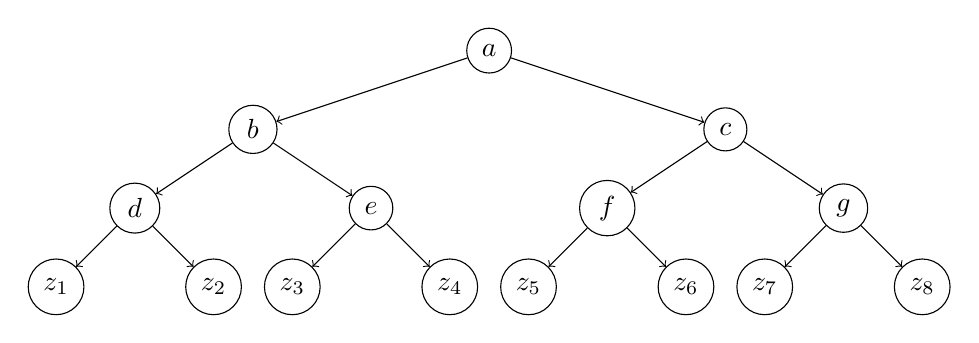
\begin{tikzpicture}[main/.style = {draw, circle}]
\node[main] (1) at (3,0){$a$};
\node[main] (2) at (0,-1) {$b$};
\node[main] (3) at (6,-1) {$c$};
\node[main] (4) at (4.5,-2) {$f$};
\node[main] (5) at (7.5,-2) {$g$};
\node[main] (6) at (-1.5,-2) {$d$};
\node[main] (7) at (1.5,-2) {$e$};
\node[main] (8) at (-2.5,-3) {$z_1$};
\node[main] (9) at (-0.5,-3) {$z_2$};
\node[main] (10) at (0.5,-3) {$z_3$};
\node[main] (11) at (2.5,-3) {$z_4$};
\node[main] (12) at (3.5,-3) {$z_5$};
\node[main] (13) at (5.5,-3) {$z_6$};
\node[main] (14) at (6.5,-3) {$z_7$};
\node[main] (15) at (8.5,-3) {$z_8$};
\draw[->] (1) -- (2);
\draw[->] (1) -- (3);
\draw[->] (3) -- (4);
\draw[->] (3) -- (5);
\draw[->] (2) -- (6);
\draw[->] (2) -- (7);
\draw[->] (6) -- (8);
\draw[->] (6) -- (9);
\draw[->] (7) -- (10);
\draw[->] (7) -- (11);
\draw[->] (4) -- (12);
\draw[->] (4) -- (13);
\draw[->] (5) -- (14);
\draw[->] (5) -- (15);
\end{tikzpicture}

(I am bad at tikzpicture so I will specify the details of the game manually). Player 1 has information sets $\{ a\}$, and $\{ d, e, f, g\}$, and player 2 acts at information set $\{ b, c \}$. All the moves are either $L$ or $R$, for both players, for left or right. The mixed strategies for player 1 are in $\Delta(\{ LL, LR, RL, RR \})$. Consider strategy $\{ 1/2, 0, 0, 1/2 \}$ for player 1, and suppose player 2 just plays strategy $L$. The mixed strategy outcome distribution is $(1/2) z_1 + (1/2) z_6$. However, any behavioral strategy that assigns nonzero probability to both $z_1$ and $z_6$  must mix at the second information set $\{ d, e ,f, g \}$,
and hence must also assign nonzero probability to $z_2$ and $z_5$, which results in a distinct outcome distribution from the mixed strategy. Hence, no behavior strategy is outcome equivalent to this mixed strategy, and we are done.

\section*{Problem 3}
Fix player $i$. Let $H_i$ denote the set of information sets, and let $A(h_i)$ denote the set of actions of player $i$ at information set $h_i \in H_i$. Then we have the set of behavioral strategies is given by
\[ \times_{h_i \in H_i} \Delta\left(A(h_i)\right)  \]
So the dimension of this is
\[ \sum_{h_i \in H_i} \left(|A(h_i)| - 1\right) \]
The set of mixed strategies is given by
\[ \Delta \left( \times_{h_i \in H_i} A(h_i) \right) \]
This has dimension
\[ \left( \prod_{h_i \in H_i} |A(h_i)| \right) - 1 \]
\section*{Problem 4}
No, consider the game where the actions of player $1$ are $A,B$ and the actions of player $2$ are $A,B$. Suppose that the outcomes are $0$ for everyone unless both players play $A$, in which case the outcomes are $1$ for everyone. No matter which player is put as moving `first' in the extensive form game, there will always be two distinct terminal nodes with outcome 0. Hence, this is a counterexample, and not any arbitrary normal form game can be written as an extensive form game with \textbf{unique} terminal nodes. 
\end{document}
	% line of code telling latex that your document is ending. If you leave this out, you'll get an error
